% !BIB TS-program = biber

\RequirePackage[l2tabu,orthodox]{nag}
% TODO: decide if one-sided/two-sided
%\documentclass[headsepline,footsepline,footinclude=false,fontsize=11pt,paper=a4,listof=totoc,bibliography=totoc,BCOR=12mm,DIV=12]{scrbook} % two-sided
\documentclass[headsepline,footsepline,footinclude=false,oneside,fontsize=11pt,paper=a4,listof=totoc,bibliography=totoc]{scrbook} % one-sided
% TODO: change thesis information
\newcommand*{\getUniversity}{Technische Universität München}
\newcommand*{\getFaculty}{Informatics}
\newcommand*{\getDegree}{Informatics}
\newcommand*{\getSchool}{Computation, Information and Technology}
\newcommand*{\getTitle}{Analysis of the Noisy Neighbor Problem in AWS}
\newcommand*{\getTitleGer}{Analyse der "Noisy Neighbor" Problem in AWS}
\newcommand*{\getAuthor}{Youssef Jemal}
\newcommand*{\getDoctype}{Bachelor's Thesis}
\newcommand*{\getSupervisor}{Prof. Dr. Leis Viktor}
\newcommand*{\getAdvisor}{Till Steinert}
\newcommand*{\getKeywords}{keyword;another keyword;one more}
\newcommand*{\getSubmissionDate}{22/08/2025}
\newcommand*{\getSubmissionLocation}{Munich}

% TODO: change citation style in settings
\PassOptionsToPackage{table,svgnames,dvipsnames}{xcolor}

\usepackage[a-2u]{pdfx} % generate PDF/A: archival compliant, self-contained pdf
\usepackage[utf8]{inputenc}
\usepackage[T1]{fontenc}
\usepackage[sc]{mathpazo}
\usepackage{diagbox}
\usepackage{float}
\usepackage[ngerman,american]{babel}
\usepackage[autostyle]{csquotes}
\usepackage[%
  backend=biber,
  url=false,
  style=numeric,
  maxnames=4,
  minnames=3,
  maxbibnames=99,
  giveninits,
  uniquename=init]{biblatex} % TODO: adapt citation style
\usepackage{graphicx}
\usepackage{scrhack} % necessary for listings package
\usepackage{listings}
\lstset{
  language=C,
  basicstyle=\ttfamily\small,
  keywordstyle=\color{blue},
  commentstyle=\color{gray},
  stringstyle=\color{orange},
  numbers=left,
  numberstyle=\tiny,
  stepnumber=1,
  numbersep=5pt,
  showstringspaces=false,
  breaklines=true,
  frame=single,
  captionpos=b,
  tabsize=4
}
\usepackage{lstautogobble}
\usepackage{tikz}
\usepackage{pgfplots}
\usepackage{pgfplotstable}
\usepackage{booktabs}
\usepackage[final]{microtype}
\usepackage[font=small,justification=centering]{caption}
\usepackage[printonlyused]{acronym}
\usepackage{ifthen}


\hypersetup{hidelinks} % removes colored boxes around references and links

% for fachschaft_print.pdf
\makeatletter
\if@twoside
	\typeout{TUM-Dev LaTeX-Thesis-Template: twoside}
\else
	\typeout{TUM-Dev LaTeX-Thesis-Template: oneside}
\fi
\makeatother

\addto\extrasamerican{
	\def\lstnumberautorefname{Line}
	\def\chapterautorefname{Chapter}
	\def\sectionautorefname{Section}
	\def\subsectionautorefname{Subsection}
	\def\subsubsectionautorefname{Subsubsection}
}

\addto\extrasngerman{
	\def\lstnumberautorefname{Zeile}
}

% Themes
\ifthenelse{\equal{\detokenize{dark}}{\jobname}}{%
  % Dark theme
  \newcommand{\bg}{black} % background
  \newcommand{\fg}{white} % foreground
  \usepackage[pagecolor=\bg]{pagecolor}
  \color{\fg}
}{%
  % Light theme
  \newcommand{\bg}{white} % background
  \newcommand{\fg}{black} % foreground
}

\bibliography{bibliography}

\setkomafont{disposition}{\normalfont\bfseries} % use serif font for headings
\linespread{1.05} % adjust line spread for mathpazo font

% Add table of contents to PDF bookmarks
\BeforeTOCHead[toc]{{\cleardoublepage\pdfbookmark[0]{\contentsname}{toc}}}

% Define TUM corporate design colors
% Taken from http://portal.mytum.de/corporatedesign/index_print/vorlagen/index_farben
\definecolor{TUMBlue}{HTML}{0065BD}
\definecolor{TUMSecondaryBlue}{HTML}{005293}
\definecolor{TUMSecondaryBlue2}{HTML}{003359}
\definecolor{TUMBlack}{HTML}{000000}
\definecolor{TUMWhite}{HTML}{FFFFFF}
\definecolor{TUMDarkGray}{HTML}{333333}
\definecolor{TUMGray}{HTML}{808080}
\definecolor{TUMLightGray}{HTML}{CCCCC6}
\definecolor{TUMAccentGray}{HTML}{DAD7CB}
\definecolor{TUMAccentOrange}{HTML}{E37222}
\definecolor{TUMAccentGreen}{HTML}{A2AD00}
\definecolor{TUMAccentLightBlue}{HTML}{98C6EA}
\definecolor{TUMAccentBlue}{HTML}{64A0C8}

% Settings for pgfplots
\pgfplotsset{compat=newest}
\pgfplotsset{
  % For available color names, see http://www.latextemplates.com/svgnames-colors
  cycle list={TUMBlue\\TUMAccentOrange\\TUMAccentGreen\\TUMSecondaryBlue2\\TUMDarkGray\\},
}

% Settings for lstlistings
\lstset{%
  basicstyle=\ttfamily,
  columns=fullflexible,
  autogobble,
  keywordstyle=\bfseries\color{TUMBlue},
  stringstyle=\color{TUMAccentGreen},
  captionpos=b
}


\begin{document}

% Set page numbering to avoid "destination with the same identifier has been already used" warning for cover page.
% (see https://en.wikibooks.org/wiki/LaTeX/Hyperlinks#Problems_with_Links_and_Pages).
\pagenumbering{alph}
\input{pages/cover}

\frontmatter{}

\begin{titlepage}
  \centering

  \IfFileExists{logos/tum-\fg.pdf}{%
    \includegraphics[height=20mm]{logos/tum-\fg.pdf}
  }{%
    \vspace*{20mm}
  }

  \vspace{5mm}
  {\huge\MakeUppercase{School of \getSchool{} --- \getFaculty{}} \par}

  \vspace{5mm}
  {\large\MakeUppercase{\getUniversity{}} \par}

  \vspace{20mm}
  {\Large \getDoctype{} in \getDegree{} \par}

  \vspace{15mm}
  {\LARGE\bfseries \getTitle{} \par}

  \vspace{10mm}
  {\LARGE\bfseries \foreignlanguage{ngerman}{\getTitleGer{}} \par}

  \vspace{15mm}
  \begin{tabular}{l l}
    Author:          & \getAuthor{}         \\
    Examiner:      & \getSupervisor{}     \\
    Supervisor:         & \getAdvisor{}        \\
    Submission Date: & \getSubmissionDate{} \\
  \end{tabular}

  \IfFileExists{logos/faculty-\fg.pdf}{%
    \vfill{}
    \includegraphics[height=20mm]{logos/faculty-\fg.pdf}
  }{}
\end{titlepage}

\input{pages/disclaimer}
%\input{pages/acknowledgments}
\input{pages/abstract}
\microtypesetup{protrusion=false}
%\tableofcontents{}
\microtypesetup{protrusion=true}

\mainmatter{}

%\input{chapters/01_introduction}
% TODO: add more chapters here
\chapter{Introduction (\checkmark)}\label{chapter:introduction}

\ac{IaaS} is a cloud computing model that provides customers with access to computing 
resources such as servers, networking and virtualization. Cloud vendors in general and \ac{AWS} in particular 
abstract the physical placement of the virtual machine providing users with limited transparency to how 
many tenants are sharing the underlying hardware. This information can be crucial as 
this co-residency can result in significant performance degradation across different resources such as 
CPU, memory, network and storage I/O \cite{characterizing_public} \cite{mitigating_resource}. 
Although virtualization technology has undergone major improvements in 
the past decades, contention can still occur due to other factors such as \ac{SMT}, Network Interface
Card queuing, and other system-level bottlenecks. To address the issue of unwanted resource 
contention, Amazon Web Services introduced dedicated hosts \cite{dedHost}, which are physical servers that are fully 
dedicated to the customer,  allowing users to deploy virtual machines with complete transparency over their
placement. Another potential solution are the spread placement groups, which ensure that the VMs are placed 
on different physical servers. It can be
particularly useful for highly parallel workloads, where the nodes have a similar workload nature
(network- or CPU-intensive). However, this approach only mitigates internal resource contention and is 
limited to a small number of EC2 instances in the same availability zone \cite{spread}. \\
In this paper, we leverage different benchmarking tools to assess the extent of the performance degradation 
that can occur because of VM co-location. We are particularly interested in quantifying the worst possible 
degradation that can happen by running identical resource-intensive benchmarks in parallel across VMs 
residing on the same dedicated host. We primarily utilized 5th and 6th general-purpose \ac{AWS} EC2 VM 
instances that are built around the \ac{AWS} Nitro system and run on top of the Nitro hypervisor. 
We analyze CPU contention across various CPU vendors namely Intel, Gravtion, and AMD. 
We examine whether and to what extent \ac{SMT} is involved in this degradation. 
Furthermore, we investigate network resource contention, which is interesting since \ac{AWS} does not provide
exact specifications like other resources such as CPU and memory. 
We analyze the degradation that can occur both on throughput and latency across co-located EC2 Instances.\\ 
The thesis is structured as follows: We start by discussing related work in section 2. 
Section 3 introduces the key concepts required to understand this work, namely virtualization and 
Simulatenous Multi Threading. In section 4, we explain the methodology of our experiments
and introduce the different benchmarking tools that were adopted throughout the thesis. 
Section 5 analyzes CPU contention across 5th and 6th EC2 generations and contexualizes the results in 
relation to the CPU architecture. In Section 6, we examine network I/O contention and 
explore its manifestation across throughput and latency. Section 7 concludes our work and summarizes 
its most important findings. 
\chapter{Related Work}\label{chapter:related}

Han et. al \cite{characterizing_public} investigated public cloud resource contention. They executed
CPU, disk, and network I/O benchmarks across up to 48 VMs sharing the same dedicated host. The tests were
executed mainly on 3rd (c3), 4th (c4), and 5th (m5d) generation VMs.  
The results showed considerable performance degradation, with CPU degradation reaching 48\%
and throughput degradation up to 94\%. Throughput degradation was measured in relation to the initial 
bandwidth available to the VM, i.e., burst bandwidth and not the baseline bandwidth. 
The paper also analyzed the 
unexpected CPU performance degradation caused by adding idle Linux VMs on the dedicated host. 
The measurements were leveraged to train multiple linear regression and random forest models to predict
VM co-residency. The linear regression model achieved an $R^2$ of .942.
This could be very practical, as it enables users to relocate their VMs to have 
access to better performance with less contention. \\
Rehman et. al \cite{initial_findings} analyzed the problem of provisioning variation in public clouds. 
By running benchmarks and sample MapReduce workloads, they found that provisioning variation can 
impact the performance by a factor of 5. They argue that this is primarily due to network I/O contention. \\
Lloyd et. al \cite{mitigating_resource} reported a 25\% performance degradation when 
running compute-intensive scientific modelling web services on pools consisting of m1.large VMs with 
high resource contention. They developed an approach called Noisy-Neighbor-Detect that leverages 
the cpuSteal metric to identify VMs with noisy neighbors from a pool of worker VMs. 
cpuSteal refers to the percentage of time a virtual CPU spends waiting for the hypervisor to allocate 
a physical CPU to run on. \\
Many other techniques were developed by researchers to identify or predict resource contention.
Govindan et. al \cite{cache_contention} developed a software solution called Cuanta 
that predicts performance interference due to shared chip-level resources, namely cache space and memory 
bandwidth. Although the performance degradation of consolidated application can be empirically
investigated, the number of possible workload placements is combinatorial. A cloud provider hosting 
$M$ VMs with $N$ VMs per server needs to perform $\frac{M!}{N!\,(M-N)!}$ measurements, which is
highly impractical. Cuanta does not require any changes to the hosting platform's software and the 
prediction complexity is linear to the number of cores sharing the Last Level Cache (LLC), 
making it a far better alternative than its empirical counterpart. 
The software provided promising results with up to 96\% accuracy on Intel Core-2-Duo processors. \\
Some efforts have looked at side channels as a way to detect VM co-location. Side channels are an indirect
way of extracting information from a system that designers never intended to expose its implementation
details. Inci et. al \cite{LLC} developed three methods to detect co-located VMs. 
The first two approaches leveraged Last Level Cache: Cooperative LLC covert channel and  
Cache profiling. While the former requires cooperation of the victim VMs, the latter operates
independently. In the second method, the attacker fills the cache with its own data and after a
short pause re-accesses the same buffer while monitoring the memory access time. Low eviction rates
indicate that the attacker is likely alone on the host, while high eviction rates point toward 
VM co-location. The third method is memory bus locking. The idea is for the attacker to launch 
special instructions that block the memory bus and then analyze the resulting delays to infer 
VM-colocation. All three methods had a high accuracy in detecting co-location in real commercial cloud
settings.

\begin{comment}
They also investigated performance variation that's caused by hardware heterogeneity
in the same instance type. They examined this trend on 12 VM types across 1st (m1, c1), 2nd (m2), 
and 3rd (c3) EC2 generationand found that 25\% of the types had more than one hardware implementation. They implemented the virtual 
machine scaler, a web services application, that helps with VM management/placement on AWS. 
It features the "forceCpuType" parameter, that allows the user to specify the backing CPU, enforcing hardware 
homogeneity. Mon-matching VMs are repeatedly terminated until the "right" CPU is allocated. 
With this, they were able to improve scientific modeling web services performance by up to 14\%.
\end{comment}
\chapter{Background}\label{chapter:background}
\section{Virtualization (\checkmark)}
Virtualization is a technology that allows the creation of isolated virtual environments also known as 
Virtual Machines that run on the same physical server \cite{virtualization_review}. Each VM has its own 
operating system and acts as an independent physical computer. The VMs are called "guests" and the 
physical server is called "host". Virtualization is crucial for the \ac{IaaS} model that's offered by 
cloud providers, as it provides various advantages \cite{virtualization_review}. It improves resource and 
cost efficiency by dividing the physical server into multiple isolated instances, each tailored to 
different workload needs. This reduces the amount of unused capacity that occurs when a server is dedicated 
to just one task. \\
The main component that handles the necessary tasks for virtualization is the \ac{VMM} 
also called hypervisor \cite{nitro_whitepaper}. Most of the instructions that are executed by the virtual 
achines run natively on the CPU and do not require intervention from the \acs{VMM}, such as arithmetic 
operations. 
However, there is a class of privileged instructions that guests can not directly execute on the CPU, 
such as I/O operations. When such an instruction is encountered, the CPU raises a 
trap, that signals to the \acs{VMM} to intervene and emulate the behavior of the instruction \cite{nitro_whitepaper}.  
After the emulation is finished, the control is then given back to the guest OS, 
which is unaware of the underyling emulation. Several optimizations techniques have been introduced 
to reduce virtualization overhead, which will be briefly outlined later. \\
Virtualization cannot be carried out by the VMM alone, as it does not virtualize hardware and therefore 
can not grant the guests access to the underlying hardware devices such as network interface, storage drives, 
and input peripherals. Device models are required for this \cite{nitro_whitepaper}. They are basically 
software components that communicate with the shared hardware and expose multiple virtual device 
interfaces to the VMs. These device models, along with other management software, run in a special 
privileged virtual machine called management domain which represents the host's operating system and 
has access to all the underlying hardware. This domain is called domain zero or dom0 in the Xen project 
and root/parent partition in the Hyper-V project \cite{nitro_whitepaper}. Since the device models are 
software-based, they compete for resources for CPU and system resources along with the existing VMs and 
can negatively affect the performance of these guests. 
The following figure summarizes the architecture of a traditional virtualization system. 
\begin{figure}[H]
  \centering
  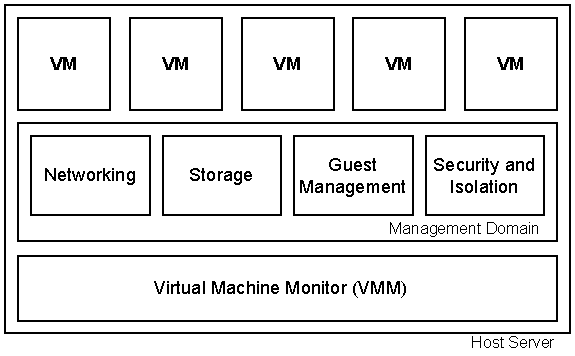
\includegraphics[width=10cm, height=6cm]{figures/traditional_hypervisor.pdf}
  \caption{Architecture of traditional virtualization Solution}
  \label{fig:hyper}
\end{figure}

\subsection{Evolution of Virtualization Solutions}
Virtualization technology has evolved significantly. It began with full software virtualization, 
where the guest OS is unmodified and "unaware" of the virtual environment. Privileged instructions 
are trapped by the CPU and the hypervisor emulates the sensitive instructions using 
binary translation \cite{virtualization_gregg}. This is, however, very slow and can make the host apps 
run 2x to 10x slower \cite{virtualization_gregg}. \\
Then paravirtualization was introduced, where the guest OS is modified to interact directly with the 
hypervisor via "hypercalls", removing the abstract emulation layer that is found in full 
software virtualization. The downside of this approach is that it introduces additional complexity, 
as it requires modifications to the guest operating system \cite{hvm}.\\ 
The next major leap was hardware assisted virtualization (HVM) which introduced virtualization support 
directly on the hardware level by providing highly efficient and fast virtualization commands. 
This provides a significant improvement in comparison to the previous virtualization 
techniques, as it reduces the involvement of the host system in handling privilege and adress translation
space tasks \cite{hvm}. Intel offers this under the Intel VT-x technology that provides virtualization of CPU and memory.
Another important example is Single Root Virtualization (SR-IOV) \cite{nitro_whitepaper}, which is a technology that allows physical 
PCIs device such as Network Interface Card (NIC) to expose multiple virtual devices to the hypervisor. 
The hypervisor can then provide the different virtual machines with direct hardware access to these virtual 
devices, which significantly increases the I/O performance. 

\subsection{The AWS Nitro System}
The Nitro System is a result of a multi-year incremental process of AWS re-imagining the virtualization 
technology in order to optimize it specifically for their EC2 data centers \cite{nitro_whitepaper}. 
The main idea was to decompose the software components, i.e., the device models, 
that run on the management domain and offload them to independent purpose-built server components. 
This helps minimize the resource usage caused by software running in the management domain, effectively 
allowing a near "bare-metal" performance. Figure \ref{fig:nitro} depicts the new AWS
architecture for virtualization \cite{nitro_whitepaper}. 
\begin{figure}[H]
  \centering
  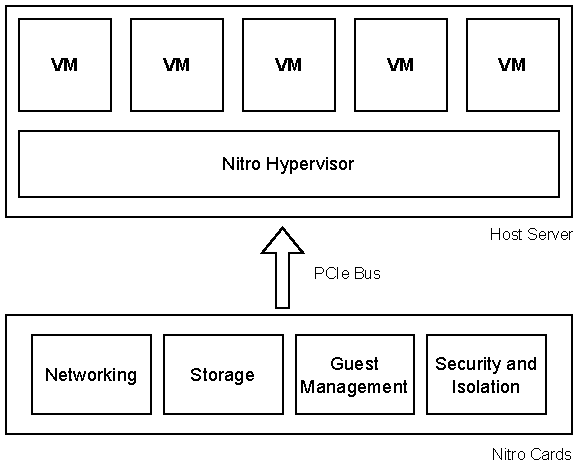
\includegraphics[width=10cm, height=7.5cm]{figures/nitro}
  \caption{Architecture of Nitro System Virtualization}
  \label{fig:nitro}
\end{figure}
\noindent
There are three main components in the AWS Nitro System \cite{nitro_whitepaper}. 
\subsubsection{The Nitro Cards}
Nitro cards are dedicated hardware components that operate independently from the EC2's server main board 
(CPU and memory) and are physically attached to it via PCIe. They "implement all the outward-facing 
control interfaces used by the EC2 service" responsible for provisioning and managing compute, memory, 
and storage \cite{nitro_whitepaper}. They provide all I/O Interfaces as well, such 
as the ones for storage and networking. These cards employ the previously explained SR-IOV technology to 
provide direct hardware interfaces to the VMs. Example of Nitro cards are Nitro cards for I/O and 
Nitro Controller, which provides the hardware root of trust of the Nitro System. 

\subsubsection{The Nitro Security Chip}
The Nitro Security Chip extends the hardware root of trust and control over the system main board. It's 
managed by the Nitro Controller and plays a crucial role in enabling 
AWS to offer bare-metal instances. Bare-metal instances provide direct access to the physical CPUs and memory 
of the physical server. They are useful mainly for licensing-restriced business critical applications, or for 
specific workloads that require direct access to the underlying infrastructure. \\ 
In virtualized environments, the hypervisor is responsible for securing the host's hardware assets. 
However, in bare metal modes, when no hypervisor is present, the Nitro Security Chip 
assumes this role and ensures the security of the system firmware from tampering attempts through the system 
CPUs \cite{nitro_whitepaper}. 

\subsubsection{The Nitro Hypervisor}
The third component is the AWS Nitro Hypervisor, which has significantly fewer responsibility than traditional
hypervisors, as most virtualization tasks are offloaded to the Nitro cards. It has three main functions.
It's responsible for partitioning memory and CPU by using the virtualization commands provided by the 
processor. It's also in charge of assigning the virtual hardware interfaces provided by 
the Nitro cards to the Virtual Machines and also handles the machine management commands that come from 
the Nitro Controller (start, terminate, stop etc.) \cite{nitro_whitepaper}. 

\section{Simultaneous Multi-threading (\checkmark)}
Before we dive deeper into \ac{SMT}, it's important to understand which problem it  
tries to solve and what the motivation behind it is. \\
A processor consists of a few hundred registers, load/store units and a couple of multiple arithmetic units. 
The main goal is to keep all these resources as busy as possible. To reach this, multiple techniques have been 
employed such as instruction pipelining, superscalar architecture and out-of-order execution 
\cite{SMT_Maximizing_on_chip_parallelism}.
Pipelining is a technique that breaks down the execution of an instruction into several distinct 
stages, with each stage using separate hardware resources \cite{SMT_under_the_hood}. During each CPU cycle, 
instructions advance from one stage to another. This allows the CPU to work on multiple instructions 
simultaneously, each being on a different stage. In a perfect scenario, where all instructions are 
independent, the processor can work simultaneously on \begin{math}n\end{math} instructions, 
with \begin{math}n\end{math} being the depth of the pipeline, i.e., the number of stages. 
The following table depicts a simple example of a five-stage pipeline. At the 5th clock cycle, 
the CPU is simultaneously working on 5 instructions.  

\begin{figure} [H]
\centering
\begin{tabular}{c|ccccccc}
\toprule
\diagbox[width=3.5cm]{Instr. No.}{Clock Cycle} 
  & \textbf{1} & \textbf{2} & \textbf{3} & \textbf{4} & \textbf{5} & \textbf{6} & \textbf{7} \\
\midrule
1 & IF  & ID  & EX  & MEM & WB  &     &     \\
2 &     & IF & ID  & EX  & MEM & WB  &     \\
3 &     &     & IF & ID  & EX  & MEM & WB  \\
4 &     &     &     & IF  & ID  & EX  & MEM \\
5 &     &     &     &    & IF  & ID  & EX  \\
\bottomrule
\end{tabular}
\caption{Basic five-stage pipeline (IF = Instruction fetch, ID = Instruction decode, EX = execute  MEM = memory read, WB = Write back to memory)}
\label{fig:table}
\end{figure}
\noindent
Modern processors are also superscalar. This means that each processor, can start executing more 
than one instruction per cycle by dispatching them to different execution units \cite{SMT_Maximizing_on_chip_parallelism}. 
Issue width is an important characteristic of modern CPUs and it represents 
the maximum number of instructions that can be started in a single clock cycle.
Although these optimizations significantly increase the processor throughput, the dependency  
between the instructions and the long latency-operations of the executing threads limit the usage of the 
available execution resources \cite{SMT_Maximizing_on_chip_parallelism}. Out-Of-Order execution partially 
solves this problem but is still not enough as it still dispatches instructions from the same thread, where 
the dependency between the instructions is inherently high. 
The wastages that occur on the processor can be categorized into two categories: Horizontal and 
vertical waste \cite{SMT_Maximizing_on_chip_parallelism}. 
Horizontal waste occurs when the CPU is not able to fully saturate the issue width of the processor. 
Vertical waste occurs when the processor is not able to start any instruction at all on a given cycle
because of the dependency to the executing instructions or delays such as memory latency. 
Traditional multithreading addresses this issue by switching to a different thread, whenever 
the currently executing one stalls.. This approach, however, only mitigates vertical waste, as 
it still issues instructions from only one thread at any given cycle \cite{SMT_Maximizing_on_chip_parallelism}.
\begin{figure}[H]
    \centering
    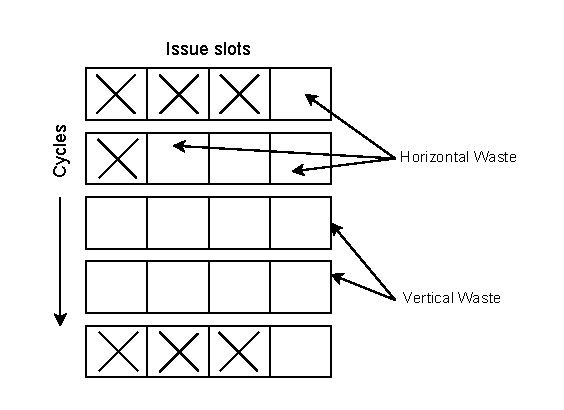
\includegraphics[width=10cm, height=7.5cm]{figures/cpu_wastages}
    \hspace{-2.5cm}
    \caption{Vertical waste vs. horizontal waste}
    \label{fig:cpu}
\end{figure}
\noindent
This is where \acl{SMT} comes into play. \acs{SMT} is a technique that helps enhance the overall efficiency of superscalar CPUs 
by improving the parallelization of computation \cite{SMT_under_the_hood}. This technology allows the 
physical core to dispatch instructions from more than one thread per cycle without requiring 
a context switch \cite{SMT_Maximizing_on_chip_parallelism}, effectively transforming each physical core into two (or more) "logical" cores. The idea is that instructions from different
threads provide greater independency, which results in a better utilization of the core's execution 
resources \cite{SMT_under_the_hood}.
To be able to achieve this, some resources of the processor are duplicated, 
e.g., those that store the architectural state such as registers and program 
counters \cite{SMT_under_the_hood}. However, the logical 
cores still share the same execution resources, which can create conflicts, especially if both threads have 
the same workload nature, e.g., both are float heavy \cite{SMT_modeling_resource_contention}. 
\begin{figure}[H]
    \centering
    \hspace*{-2cm} 
    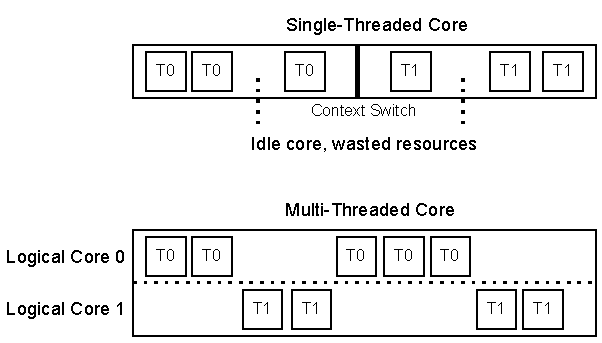
\includegraphics[width=10cm, height=6cm]{figures/single_vs_multithreaded}
    \caption{Single-Threaded Core vs. Multi-Threaded Core}
    \label{fig:all}
\end{figure}
\noindent
Both Intel and AMD implement this technology in their modern CPUs, providing two threads per physical core. 
Intel brands it as Hyper-Threading, while AMD uses the standard term \ac{SMT}. In the AWS dedicated hosts that run on an Intel or 
AMD CPU with hyperthreading enabled, the number of vCPUs is always equal to the double of the number of 
physical cores, with each vCPU corresponding to a hyperthread. This, however, opens up the possibility 
for CPU contention, if two virtual machines have access to vCPUs that share the same underlying physical core. 
Unlike Intel and AMD CPUs, AWS-designed Graviton processors, built around the ARM architecture, 
do not support hyper-threading and expose one execution context, i.e., vCPU for 
each physical core \cite{graviton}. This allows for a better isolation between the different tenants as 
there is no resource sharing between the different vCPUs apart from the last level cache and the memory 
system \cite{graviton}. 

\chapter{Methodology}

\section{Network I/O Benchmarking}
\subsection{Throughput}
For network I/O stress, we used iPerf3 \cite{iperf}. It provides a benchmark for measuring network 
bandwidth. It supports various protocols and can be used to test TCP, UDP, and SCTP 
throughput.  The tool probes the maximum achievable network bandwidth by transmitting a large number 
of packets until reaching the thoughput's upper bound. In our experiments, we measured the 
maximum UDP throughput between clients and servers. We made this choice in order to avoid congestion 
effects that can be caused by TCP congestion control, which could reduce the throughput even though 
there still might be bandwidth available. 
\subsection{Latency}
For latency benchmarking, we used the sockperf tool \cite{sockperf}, which is a network benchmarking 
utility that can measure the latency of packets at a sub-nanosecond resolution. 
This tool introduces very low overhead as it uses Time Stamp Counter (TSC) registers that count 
the number of CPU cycles for measuring latency. We ran the command with the ping-pong argument on the 
client side and with the server argument on the server side.

\section{Testing Infrastructure}
All tests were performed in the AWS us-east-1 Ohio region. The EC2 instances ran Ubuntu Server 24.04 LTS
Linux. For each experiment, all the VMs were provisioned in the same availability zone and resided
in the same Virtual Private Cloud. This is particularly important for network I/O experiments, as 
the network traffic between VMs sharing the same AZ and VPC is free of charge. We ran parallel 
benchmarks on general-purpose and compute-intensive dedicated hosts from the 5th, 6th 
and 7th generations. We used mutliple instance types varying from large to 8xlarge instances.
To deploy the resources for the different experiments, we used Terraform which is an \ac{IaC} tool 
that's developed by HashiCorp and can be used to define and provision resources using the \ac{HCL}, 
ensuring the automation and reproducibility of the benchmarks. 
Additionally, we used distexprunner \cite{distex}, which is a tool written in python 
that helps write and run bash commands remotely across multiple nodes addressing them through 
their public IPs. Our experiments generated JSON or csv files that were gathered in an S3 
bucket using distexprunner. We also implemented multiple scripts in Python3 using mainly the re 
package \cite{re} for parsing raw data and csv \cite{csv} for working with comma separated data.

\chapter{CPU Contention}

\section{Methodology (\checkmark)}
To generate CPU stress, we used sysbench \cite{sysbench}, which is a powerful cross-architecture tool
that can be used for Linux performance benchmarks. As a CPU stress-testing tool, it deterministically 
checks all prime numbers up to 10,000 (default value) by dividing each candidate number by all integers 
from 2 up to its square root \cite{gentoo_sysbench}. The number of worker threads 
as well as the aggregated workload of the created threads can be specified as arguments. 
The total execution runtime is then used as a comparison metric 
between the different experiments. For comparison purposes, we also developed our CPU stressing 
tool called \textit{cpu\_burn} written in the C language. The program takes two arguments, the first 
being the number of operations that each created thread will perform, and the second representing 
the number of worker threads. It outputs the total wall-clock runtime that was needed for the 
execution of this job. 
We compiled the program using GCC with optimization level -O0, to ensure no compiler optimizations
altered the program's behavior. Each thread executes the function defined under \texttt{perform\_work()}. 
As stated previously, The argument \texttt{work->operations} is specified by the user.

\begin{figure}[H]
\begin{lstlisting}[caption={Workload of the cpu\_burn tool}]
void* perform_work(void* arg) {
    ThreadWork* work = (ThreadWork*)arg;
    double x = 0.0;
    for (long long i = 0; i < work->operations; ++i) {
        x += i * 0.000001;
    }
    work->result = x;
    return NULL;
}
\end{lstlisting}
\end{figure}
\noindent
This section investigates CPU contention on general-purpose instances from 5th and 6th EC2 generations, 
with different CPU architectures. We analyzed the potential degradation on hosts that support 
\acl{SMT}: namely m5, m6i and m6a hosts. We then considered the single-threaded AWS Graviton 2 
processor used by the m6g dedicated host. Key Performance Indicators are described 
in Table \ref{tab:dedicated-hosts}. We notice that the first three dedicated hosts have a number of vCPUs 
twice the number of the physical cores, as these hosts support \ac{SMT} with 
two threads per physical core. The m6g instance has the best price per vCPU ratio, although each 
vCPU is mapped to a physical and not to a logical core.

\renewcommand{\arraystretch}{1.5} % Adjust this value as needed
\begin{table}[h]
\centering
\begin{tabular}{|l|p{2cm}|p{2cm}|p{2cm}|p{2cm}|}
\hline
KPI & m5 & m6i & m6a & m6g \\
\hline
Processor \cite{cloudspecs} & Intel Xeon Platinum 8175/ Intel Xeon Platinum 8280	 & Intel Xeon 8375C & AMD EPYC 7R13 Processor & AWS Graviton2 \\
\hline
Hypervisor \cite{awsEC2GP2025} & Nitro v2 & Nitro v4 & Nitro v4 & Nitro v2 \\
\hline
vCPUs \cite{pricing} & 96 & 128 & 192 & 64 \\
\hline
Physical CPUs \cite{pricing} & 48 & 64 & 96 & 64 \\
\hline
Clock speed (GHz) \cite{vantage} & 3.1 & 3.5 & 3.6 & 2.5\\
\hline
Hypervisor \cite{hypervisorSpec} & Nitro & Nitro & Nitro & Nitro \\
\hline
price/hour \cite{pricing} & \$5.069 & \$6.758 & \$9.124 & \$2.71 \\
\hline
price/vCPU/hr & \$0.053 & \$0.053 & \$0.048 & \$0.042 \\
\hline
\end{tabular}
\caption{KPIs for AWS Dedicated Host families m5, m6i, m6a, and m6g.}
\label{tab:dedicated-hosts}
\end{table}
\noindent
The experiment is structured as follows: A node, referred to as test node 
is first deployed on the dedicated host. Next, neighbors that fully utilize their vCPUs are 
incrementally added. We analyze the effect of adding busy neighbors on the runtime of running 
cpu benchmarks on the test node.
Figure \ref{fig:cpu_exp} provides a visualization of the experiment. 
\begin{figure}[H]
  \centering
  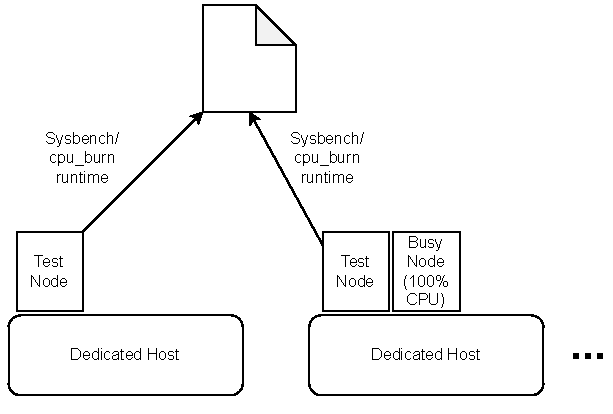
\includegraphics[width=11cm, height=7cm]{figures/cpu_exp}
  \caption{CPU contention experiment}
  \label{fig:cpu_exp}
\end{figure}
\noindent
For comparison, the experiment was repeated but with idle neighbors instead of busy. In order 
to interpret the results better, we also natively ran the benchmarking tools on the metal 
instance of each family. Metal instances run directly on the physical host without the need 
for the hypervisor. They provide the user with access to all the physical 
CPUs. The behavior of the metal instance will not be analyzed in depth, 
as it is out of the scope of the thesis. It is included solely to support a better understanding of 
CPU contention.

 
\section{Contention under SMT}
\subsection{m5 family}
The first set of experiments will be conducted on an m5 dedicated host. This host features either the 
1st or 2nd generation Intel Xeon Platinum 8000 Series processor, namely Skylake-SP or Cascade Lake 
\cite{aws_m5_instances}. The following table provides an overview of the 
different instance types that belong to this family. 
\begin{table}[H]
\centering
\begin{tabular}{lcc}
\hline
\textbf{Instance Size} & \textbf{vCPU} & \textbf{Memory (GiB)} \\
\hline
m5.large     & 2  & 8    \\
m5.xlarge    & 4  & 16   \\
m5.2xlarge   & 8  & 32   \\
m5.4xlarge   & 16 & 64   \\
m5.8xlarge   & 32 & 128  \\
m5.12xlarge  & 48 & 192  \\
\hline
\end{tabular}
\caption{m5 Instance Specifications \cite{aws_m5_instances}}
\end{table}
\noindent
The m5 dedicated host used the 2nd-generation Intel CPU in all our experiments. 
We repeated the benchmarks using hosts running on the 1st-generation CPU and we received the same
behavior, which excludes variation caused by hardware heterogeneity. 
For our first experiment, we used 2xlarge instances, each featuring 8vCPUs and 32 GiB RAM. 
The maximum number of nodes is 12. The results can 
be seen in Figure \ref{fig::m5.2xlarge_busy}

\begin{figure}[H]
\centering
\begin{tikzpicture}
\begin{axis}[
    width=12cm,
    height=7cm,
    xlabel={Number of Neighbors},
    ylabel={\% of Performance Degradation},
    grid=both,
    xtick={0,...,11},
    enlargelimits=0.05,
    legend style={at={(0.5,-0.25)}, anchor=north, legend columns=2}
]


\addplot[
    color=red,
    mark=square*,
    thick
] coordinates {
    (0, 0)
    (1, 1.65)
    (2, 1.65)
    (3, 1.65)
    (4, 1.65)
    (5, 1.65)
    (6, 3.27)
    (7, 4.98)
    (8, 4.98)
    (9, 4.98)
    (10, 4.98)
    (11, 4.98)
};

\addplot[
    color=green,
    mark=square*,
    dashed,
    thick
] coordinates {
    (0, 0)
    (1, 1.64)
    (2, 1.64)
    (3, 1.64)
    (4, 1.64)
    (5, 1.64)
    (6, 3.32)
    (7, 5)
    (8, 5)
    (9, 5)
    (10, 5)
    (11, 5)
};
\addlegendentry{sysbench}

\addlegendentry{cpu\_burn}


\end{axis}
\end{tikzpicture}
\caption{Effect of adding busy neighbors on the CPU speed of the sysbench and cpu\_burn command on the 
test node using m5.2xlarge instances}
\label{fig::m5.2xlarge_busy}
\end{figure}
\noindent
We notice a very similar degradation pattern for the two tools we used.
Adding the first neighbor added a performance degradation of  1.6\% on our test node. The runtime then 
remained constant for the next four neighbors. Afterwards, the sixth neighbor degraded the performance
further to 3.3\%. The seventh neighbor introduced the last witnessed decrease in the performance to 
reach 5\% in both experiments. \\ 
This experiment alone does not allow us to pinpoint the reason behind the performance degradation.
Potential reasons could be physical core co-location between the neighbors and the test node or 
hypervisor overhead. The latter is very unlikely, as the Nitro system, along with hardware-assisted 
virtualization should introduce a very small overhead. 
We repeat the same experiment but, we add idle VMs this time. 
Figure \ref{fig::m5.2xlarge_idle} summarizes the results. 

\begin{figure}[H]
\centering
\begin{tikzpicture}
\begin{axis}[
    width=12cm,
    height=7cm,
    xlabel={Number of Neighbors},
    ylabel={\% of Performance Degradation},
    grid=both,
    xtick={0,...,11},
    enlargelimits=0.05,
    legend style={at={(0.5,-0.25)}, anchor=north, legend columns=2}
]


\addplot[
    color=red,
    mark=square*,
    thick
] coordinates {
    (0, 0)
    (1, 1.65)
    (2, 1.65)
    (3, 1.65)
    (4, 1.65)
    (5, 1.65)
    (6, 3.27)
    (7, 5)
    (8, 5)
    (9, 5)
    (10, 5)
    (11, 5)
};

\addplot[
    color=green,
    mark=square*,
    dashed,
    thick
] coordinates {
    (0, 0)
    (1, 1.64)
    (2, 1.64)
    (3, 1.64)
    (4, 1.64)
    (5, 1.64)
    (6, 3.32)
    (7, 5)
    (8, 5)
    (9, 5)
    (10, 5)
    (11, 5)
};
\addlegendentry{sysbench}

\addlegendentry{cpu\_burn}
\end{axis}
\end{tikzpicture}
\caption{Effect of adding idle neighbors on the CPU speed of the sysbench and cpu\_burn command on the test node using m5.2xlarge hosts} 
\label{fig::m5.2xlarge_idle}
\end{figure}
\noindent
We notice the exact same degradation pattern of the earlier experiment. This result is unexpected
and undermines the hypothesis that the performance degradation is due to physical core co-location between the different 
tenants as we would have expected the effect to be less pronounced when adding idle VMs. \\
To investigate this further, we repeat the experiment using m5.large instances, of which the dedicated host can 
provision 48. The results of our experiment can be seen in Figure \ref{fig::m5.large}. In this 
case as well, adding busy or idle neighbors provided the exact same results.  

\begin{figure}[H]
\centering
\begin{tikzpicture}
\begin{axis}[
    width=12cm,
    height=7cm,
    xlabel={Number of Neighbors},
    ylabel={\% of Performance Degradation},
    grid=both,
    ymax=15, 
    xtick={0,4,8,12,16,20,24,28,32,36,40,44,47},
    enlargelimits=0.05,
    legend style={at={(0.5,-0.25)}, anchor=north, legend columns=2}
]

\addplot[
    color=red,
    thick
] coordinates {
    (0, 0.00)
    (1, 0.00)
    (2, 6.13)
    (3, 6.13)
    (4, 9.48)
    (5, 9.48)
    (6, 9.48)
    (7, 9.48)
    (8, 9.48)
    (9, 9.48)
    (10, 9.48)
    (11, 9.48)
    (12, 9.48)
    (13, 9.48)
    (14, 9.48)
    (15, 9.48)
    (16, 9.48)
   (17, 9.48)
   (18, 9.48)
   (19, 9.48)
   (20, 9.48)
(21, 9.48)
(22, 9.48)
(23, 9.48)
(24, 9.48)
(25, 9.48)
(26, 9.48)
(27, 9.48)
(28, 13)
(29, 13)
(30, 13)
(31, 13)
(32, 13)
(33, 13)
(34, 13)
(35, 13)
(36, 13)
(37, 13)
(38, 13)
(39, 13)
(40, 13)
(41, 13)
(42, 13)
(43, 13)
(44, 13)
(45, 13)
(46, 13)
(47, 13)

};
\addlegendentry{sysbench}

\addplot[
    color=green,
    dashed,
    thick
] coordinates {
    (0, 0.00)
(1, 0.00)
(2, 6.09)
(3, 6.09)
(4, 9.35)
(5, 9.35)
(6, 9.35)
(7, 9.35)
(8, 9.35)
(9, 9.35)
(10, 9.35)
(11, 9.35)
(12, 9.35)
(13, 9.35)
(14, 9.35)
(15, 9.35)
(16, 9.35)
(17, 9.35)
(18, 9.35)
(19, 9.35)
(20, 9.35)
(21, 9.35)
(22, 9.35)
(23, 9.35)
(24, 9.35)
(25, 9.35)
(26, 9.35)
(27, 9.63)
(28, 13.02)
(29, 13.02)
(30, 13.02)
(31, 13.02)
(32, 13.02)
(33, 13.02)
(34, 13.02)
(35, 13.02)
(36, 13.02)
(37, 13.02)
(38, 13.02)
(39, 13.02)
(40, 13.02)
(41, 13.02)
(42, 13.02)
(43, 13.02)
(44, 13.02)
(45, 13.02)
(46, 13.02)
(47, 13.02)

};

\addlegendentry{cpu\_burner}

\end{axis}
\end{tikzpicture}
\caption{Effect of adding busy/idle neighbors on the CPU speed of the sysbench and cpu\_burn command on 
the test node using m5.large instances}
\label{fig::m5.large}
\end{figure}

\noindent
In this experiment as well, we notice the same performance degradation between the two tools. The second 
neighbor has introduced the first performance degradation of roughly 6\%. The 4th neighbor increased 
this degradation to 9,5\%. The runtime then remained constant for the next 23 neighbor, as they had no 
effect on our test node. The 28th neighbor then introduced the last performance degradation reaching the 
maximum performance degradation of 13\% with both tools. \\
To have a full picture of the performance degradation across the different instance types, we repeated 
the experiment using the remaining instance types and summarized the results in table \ref{tab::all_m5}.
The results are always similar between the two tools. From this point, we'll only prcoceed 
with the cpu\_burn tool. Adding idle or busy neighbors constantly provided the same results. 
\begin{table}[H]
\centering
\begin{tabular}{ |c|c|c|c|c|c|c }
 Instance type & large & xlarge & 2xlarge & 4xlarge  & 12xlarge  \\
 \hline
 Maximum Nodes & 48 & 24 & 12 & 6 & 2 \\
 \hline
Degradation (Busy/Idle) \% & 13 & 13 & 4.8 & 3.25 & 0  \\ 

\end{tabular}
\caption{Maximum achievable performance degradation on our test node across various m5 instance types}
\label{tab::all_m5}
\end{table}
\noindent
The biggest performance degradation happens when using large and xlarge instances with almost the same 
percentage of 13\%. It then drops to 5\% for the 2xlarge type, as seen in figure \ref{fig::m5.2xlarge_busy}.
We notice a further decrease in the performance degradation for the 4xlarge type to 3.25\% and then its complete 
absence when using the 12xlarge type, of which the dedicated host can only provision 2. \\
DISCUSSION \\ 
In their paper, Han et. al. \cite{contention} argue that this CPU performance degradation is due to CPU 
context switching overhead that's caused by the KVM (Nitro) scheduler. Even though this hypothesis 
seems convincing, since the degradation decreases as the number of tenants decreases (Table 2), 
We think that it's very unlikely, as the Nitro System should provide a near bare-metal performance. \\
DISCUSSION \\
To investigate this issue further we run the experiment directly on the bare-metal m5.instance. 
For this, we use the cpu\_burn tool and incrementally increase the number of threads that are created 
and examinewhether we witness any performance degradation. Figure \ref{fig::m5_metal} visualizes 
the outcome of the experiment. 
\begin{figure}[H]
\centering
\begin{tikzpicture}
\begin{axis}[
    width=12cm,
    height=7cm,
    xlabel={Number of Threads},
    ylabel={\% Performance Degradation},
    grid=both,
    xtick distance=8,
    enlargelimits=0.05,
    legend style={at={(0.5,-0.25)}, anchor=north, legend columns=2}
]

\addplot[
    color=green,
    mark=square*,
    thick
] coordinates {
    (1, 0)
    (8, 9.29)
    (16, 9.46)
    (24, 9.47)
    (32, 9.46)
    (40, 11.67)
    (48, 13.2)
    (56, 42.74)
    (64, 42.74)
    (72, 45.46)
    (80, 51.66)
    (88, 53.6)
    (96, 53.6)
};


\end{axis}
\end{tikzpicture}
\caption{Runtime impact of incrementally increasing threads in the cpu\_burn command on an m5.metal instance} 
\label{fig::m5_metal}
\end{figure}
\noindent
Although the m5.metal has 96 vCPUs i.e., logical cores, we 
notice a very important pattern of performance degradation throughout the first 96 threads reaching 53\%. 
This is caused by the physical core co-location that happens between the different 
threads, resulting in resource contention, as the execution resources are not duplicated. 
We also notice a very interesting point. In all our previous experiments, the instances 
initially started with a nominal baseline performance significantly worse than running the 
exact number of threads directly on the metal instance. Figure \ref{fig::metal_vs_VMs} compares 
the runtime of cpu\_burner on the test node (all threads are busy) as we keep adding fully busy 
neighbors, in comparison to running the same number of busy threads directly on the m5.metal. 
\begin{figure}[H]
\begin{tikzpicture}
\begin{axis}[
    width=13cm,
    height=8cm,
    ylabel={Execution Runtime},
    xlabel={Number of Busy Threads},
    grid=major,
    xmin=0, 
    xmax=98,
    xtick distance= 8,
    legend pos=south east
]
\addplot[
    color=blue,
    mark=*,
] coordinates {
    (2, 5.162)
    (4, 5.471)
    (6, 5.474)
    (8, 5.638)
    (10, 5.644)
    (12, 5.647)
    (14, 5.647)
    (16, 5.651)
    (18, 5.650)
    (20, 5.649)
    (22, 5.653)
    (24, 5.650)
    (26, 5.653)
    (28, 5.653)
    (30, 5.652)
    (32, 5.654)
    (34, 5.651)
    (36, 5.651)
    (38, 5.653)
    (40, 5.658)
    (42, 5.835)
    (44, 5.836)
    (46, 5.836)
    (48, 5.836)
    (50, 7.308)
    (52, 7.356)
    (54, 7.361)
    (56, 7.362)
    (58, 7.371)
    (60, 7.368)
    (62, 7.370)
    (64, 7.373)
    (66, 7.376)
    (68, 7.407)
    (70, 7.434)
    (72, 7.5)
    (74, 7.804)
    (76, 7.81)
    (78, 7.815)
    (80, 7.82)
    (82, 7.829)
    (84, 7.858)
    (86, 7.915)
    (88, 7.92)
    (90, 7.92)
    (92, 7.928)
    (94, 7.93)
    (96, 7.93)
};

\addlegendentry{m5.metal}
\addplot[
    color=red,
    mark= *,
    thick,
] coordinates {
    (2, 7.06)
(4, 7.06)
(6, 7.49)
(8, 7.49)
(10, 7.72)
(12, 7.72)
(14, 7.72)
(16, 7.72)
(18, 7.72)
(20, 7.72)
(22, 7.72)
(24, 7.72)
(26, 7.72)
(28, 7.72)
(30, 7.72)
(32, 7.72)
(34, 7.72)
(36, 7.72)
(38, 7.72)
(40, 7.72)
(42, 7.72)
(44, 7.72)
(46, 7.72)
(48, 7.72)
(50, 7.72)
(52, 7.72)
(54, 7.72)
(56, 7.74)
(58, 7.98)
(60, 7.98)
(62, 7.98)
(64, 7.98)
(66, 7.98)
(68, 7.98)
(70, 7.98)
(72, 7.98)
(74, 7.98)
(76, 7.98)
(78, 7.98)
(80, 7.98)
(82, 7.98)
(84, 7.98)
(86, 7.98)
(88, 7.98)
(90, 7.98)
(92, 7.98)
(94, 7.98)
(96, 7.98)
 };
 \addlegendentry{m5.large}

 \addplot[
    color=green,
    mark=*,
] coordinates {
(48, 7.98)
(96, 7.98)
 };
 \addlegendentry{m5.12xlarge}
\end{axis}
\end{tikzpicture}
\caption{Performance of the test node in comparison to running the threads natively on m5.metal}
\label{fig::metal_vs_VMs}
\end{figure}
\noindent
The first two threads finished the execution in 5.165s on the bare metal instance. However, the 
first m5.large instance that  was deployed on the dedicated host took 7.06s to 
finish, even though it introduced the first two busy threads on the dedicated host and no other VMs exists.
This is highly unexpected as we would have expected to see a runtime closer to 5.165s that confirms 
the promises of AWS of a near bare-metal performance. Instead we notice a difference of almost 36.6\%. 
The same is true for the first m5.12xlarge instance where we witness a difference of 36.7\%. Furthermore, we notice that both plots converge almost towards the same value at 
the maximum number of threads. This strongly undermines the hypothesis that the degradation is due to 
hypervisor overhead as we would expect to see an even bigger gap (in relation to bare-metal) as 
more VMs are deployed on the dedicated host. The results for the performance degradation we saw in 
the previous experiments (Table 2) can be misleading. For bigger instances, we saw a relatively small 
degradation compared to the smaller instances (large and xlarge). The reason behind this is that the 
first 12xlarge instance started with a baseline performance that's 13\% worse than the performance 
of the first m5.large instance as Figure \ref{fig::metal_vs_VMs} shows. \\
The poor initial performance of the first m5.large instance (test node) suggests that the hypervisor 
pinned its vCPUs to the same physical core, not taking advantage of other non-occupied physical cores. 
We assume that this allocation technique aims to avoid contention between the different tenants/customers 
and isolate the vCPUs of each virtual machine by allocating each pair to the same physical core. 
This could be advantageous when the customer rents a unique VM, as it is independent of the neighbors’ 
workloads. However, it is highly unfavorable when the user has access to a dedicated host, as they 
are unable to fully utilize the available idle CPU resources of the physical machine, despite paying 
for all of them. \\
To confirm our supposition, we run the cpu\_burner tool in a m5.2xlarge instance, and incrementally 
increase the number of busy threads. The results can be seen in the following figure. 
\begin{figure}[H]
\centering
\begin{tikzpicture}
\begin{axis}[
    width=12cm,
    height=7cm,
    xlabel={Number of Threads},
    ylabel={\% Performance Degradation},
    grid=both,
    enlargelimits=0.05,
    legend style={at={(0.5,-0.25)}, anchor=north, legend columns=2}
]

\addplot[
    color=green,
    mark=square*,
    thick
] coordinates {
    (1, 0)
    (2, 0.07)
    (3, 0.2)
    (4, 0.2)
    (5, 26.95)
    (6, 26.94)
    (7, 34)
    (8, 36.5)
};


\end{axis}
\end{tikzpicture}
\caption{Effect of adding busy threads on the CPU performance using m5.2xlarge and the cpu\_burn tool} 
\end{figure}
\noindent
We can notice that the biggest degradation happens when adding the 5th thread, which strongly indicates 
that the instance has access to only 4 physical cores. The hypervisor starts by initially pinning the 
first 4 threads to an idle physical core to maximize performance but then the 5th thread is allocated 
to one of these physical cores, sharing the execution resources with another busy thread resulting in 
a performance degradation of 27\%.  \\
\subsubsection{Performance variation of random m5.large instances}
We wanted to analyze the variation of the performance of different m5.large instances. For this we 
sequentially launched 50 m5.large instances across different zones of the us-east-2 region to see where their 
execution runtime is situated in relation to figure \ref{fig::metal_vs_VMs}. The runtime across all the subjects
was consistently 7.98 seconds. This consistency strongly suggests that AWS pre-provisions idle instances on 
internally managed dedicated hosts even before they're rented, enabling faster boot times 
when a customer actually rents a VM. If this were not the case, then we would have expected to see 
execution runtimes around  7, 7.5 or 7.7 seconds which correspond to the three performance 
levels we witnessed on figure \ref{fig::metal_vs_VMs}. 

\subsection{m6i family}
It's interesting to see whether and to what extent the behavior we saw in the m5 family is present on 
the m6i family. The m6i family runs on the 3rd Generation Intel Xeon Scalable processor. 
We investigated the maximum performance degradation that can happen on the test nodes from adding 
idle and busy VMs with different instance types. 
\begin{table}[H]
\begin{center}
\begin{tabular}{ |c|c|c|c|c|c }
 Instance type & large & xlarge & 2xlarge & 4xlarge \\
 \hline
 Maximum Nodes & 64 & 32 & 16 & 8  \\
 \hline
Degradation (Busy) \% & 1.48 & 1.6 & 1.74 & 2.3  \\ 
\hline 
Degradation (Idle) \% & 0.05 & 0.06 & 0.06 & 0.07  \\ 
\end{tabular}
\end{center}
\caption{Maximum achievable performance degradation on our test node across various m6i instance types}
\label{tab::max_m6i}
\end{table}
\noindent
The difference from the previous experiments with the m5 family is that we notice a difference between 
adding idle or busy neighbors. Adding idle neighbors always results in a sub 0.1\% performance 
degradation which is practically insignificant. This difference between busy and idle instances can't be 
assigned to hypervisor overhead alone as we notice a sub 0.1\% overhead when adding busy instances
on the m6g dedicated host that uses the same Nitro v2 Hypervisor.\\
These series of experiments can be misleading in 
suggesting that the performance degradation for the m6i family is better than m5 seeing the percentages. 
However, in these experiments, all the instance types started from nearly the same nominal performance 
level, which is roughly 2\% away from the highest runtime possible on the metal instance (128 busy 
threads). This explains the small levels of performance degradation we witnessed in comparison to the m5 family 
where the m5.large and m5.xlarge instances started with a relatively better (nominal) performance than 
the other types resulting in a bigger performance degradation in comparison to the other types. 
We now analyze the execution runtime of busy threads directly on the m6i.metal instance, in comparison
to to the test node while adding busy 4xlarge neighbors. At 128 threads, both the m6i metal and the 
test nodes had the same execution runtime, which supports the claim that the difference between 
busy and idle neighbor in Table \ref{tab::max_m6i} is not solely due to hypervisor overhead.  

\begin{figure}[H]
\begin{tikzpicture}
  \begin{axis}[
    width=13cm,
    height=8cm,
    ylabel={Execution Runtime},
    xlabel={Number of Busy Threads},
    grid=major,
    xmin=0, 
    xmax=132,
    xtick distance= 8,
    legend pos=south east
  ]
    \addplot[
      color=blue,
      mark=*,
    ]
    coordinates {
      (1, 5.150)
      (8, 5.159)
      (16, 5.160)
      (24, 5.159)
      (32, 5.166)
      (40, 5.166)
      (48, 5.164)
      (56, 5.169)
      (64, 5.168)
      (65, 6.248)
      (72, 6.257)
      (80, 6.262)
      (88, 6.270)
      (96, 6.457)
      (104, 6.490)
      (112, 6.508)
      (120, 6.554)
      (128, 6.68)
    };

    \addplot[
      color=red,
      mark=*,
    ]
    coordinates {
      (16, 6.54)
      (32, 6.54)
      (48, 6.54)
      (64, 6.64)
      (80, 6.64)
      (96, 6.64)
      (112, 6.64)
      (128, 6.69)
    };
\addlegendentry{m6i.metal}
\addlegendentry{m6i.4xlarge}

\end{axis}
\end{tikzpicture}
\caption{Performance of the test node in comparison to running the threads natively on m6i.metal}
\end{figure}
\noindent
We notice the same behavior we witnessed on 1st gen and 2nd gen Intel Xeon Scalable processor from the 
m5.family. We notice that in both the m5.metal and m6i.metal, the most significant performance degradation 
happens exactly at    \begin{math}n / 2 + 1\end{math} with n being the maximum number of vCPUs available 
to the dedicated host. Our hypothesis is that the first \begin{math}n/2\end{math} threads are scheduled 
each on an independent physical core. However the \begin{math}n / 2 + 1\end{math} thread needs to share 
a physical core with another thread, as explained previously. This results in the performance degradation 
of 20.9\% we witness here and 25.22\% using m5.metal. The maximum performance degradation using this 
m6i.metal is less than m5.metal, reaching 31.85\% here in comparison to 53\%. Over the first 64 
threads (\begin{math}n/2\end{math}), we notice very small performance degradation of 0.35\%, in 
comparison to 13.2\% on the m5.metal instance (over the first 48 threads). In this experiment as well, 
we notice that the the first m6i.4xlarge has an intial performance 26.7\% worse than deploying the 
threads natively on the bare-metal instance. We assume that the same vCPU distribution happens with this 
host as explained for the m5 host. \\
We investigate whether this behavior also exists on processors from other vendors 
that support multi-threading such as some AMD processors.
\subsection{m6a family}
The m6a host features the AMD EPYC 7R13 Processor that also support \ac{SMT} with two threads per core.

\begin{table}[H]
\begin{center}
\begin{tabular}{ |c|c|c|c|c|c }
 Instance type & large & xlarge & 2xlarge & 4xlarge \\
 \hline
 Maximum Nodes & 96 & 48 & 24 & 12  \\
 \hline
Degradation (Busy) \% & 10 & 9.5 & 11.1 & 11.4  \\ 
\hline 
Degradation (Idle) \% & 0.05 & 0.06 & 0.06 & 0.05  \\ 
\end{tabular}
\end{center}
\caption{Maximum achievable performance degradation on our test node across various m6i instance types}
\label{tab::max_m6a}
\end{table}


\begin{figure}[H]
\begin{tikzpicture}
\begin{axis}[
    width=13cm,
    height=8cm,
    ylabel={Execution Runtime},
    xlabel={Number of Busy Threads},
    grid=major,
    xmin=0, 
    xmax=192,
    xtick distance= 16,
    legend pos=south east
]

\addlegendentry{m6a.metal}
\addplot[
    color=blue,
    mark= *,
    thick,
] coordinates {
(1, 6.47)
(16, 6.50)
(32, 6.70)
(48, 6.70)
(64, 6.71)
(80, 6.72)
(96, 6.72)
(97, 7.06)
(112, 7.20)
(128, 7.34)
(144, 7.51)
(160, 7.67)
(176, 7.88)
(192, 7.9)
 };

\addlegendentry{m6a.4xlarge}
\addplot[
    color=green,
    mark= *,
    thick,
] coordinates {
(16, 7.09)
(32, 7.09)
(48, 7.09)
(64, 7.09)
(80, 7.09)
(96, 7.09)
(112, 7.09)
(128, 7.43)
(144, 7.44)
(160, 7.44)
(176, 7.90)
(192, 7.91)
 };

\end{axis}
\end{tikzpicture}
\caption{Performance of the test node in comparison to running the threads natively on m5.metal}
\label{fig::m6a_metal_vs_VMs}
\end{figure}
\noindent
We notice a pattern similiar to that of the Intel processors. However the final performance degradation is 
less important and is equal to 23.5 \%. When adding the 97th ($n/2 + 1$) busy thread, we witness a degradation 
of 5.2\%, which is not very important in comparison to the m5 and the m6i dedicated hosts. 
We notice that the biggest part of the degradation happens in the second half of adding the 
busy threads, i.e., from thread 97 to 192. We see almost a steady upwards increasing line. 
\subsection{m6a Family}
The m6a host features the AMD EPYC 7R13 Processor. Table \ref{tab::max_m6a} captures the maximum 
achievable performance degradation on the test node while adding busy or idle neighbors. 

\begin{table}[H]
\begin{center}
\begin{tabular}{ |c|c|c|c|c|c }
 Instance type & large & xlarge & 2xlarge & 4xlarge \\
 \hline
 Maximum Nodes & 96 & 48 & 24 & 12  \\
 \hline
Degradation (Busy) \% & 10 & 9.5 & 11.1 & 11.4  \\ 
\hline 
Degradation (Idle) \% & 0.05 & 0.06 & 0.06 & 0.05  \\ 
\end{tabular}
\end{center}
\caption{Maximum achievable performance degradation on our test node across various m6i instance types}
\label{tab::max_m6a}
\end{table}
\noindent
When adding busy neighbors, we notice close percentages of performance 
degradation across the different instance types,  with an average of 10\%. 
When alone on the dedicated host, the test node started from roughly the same initial nominal value 
across all the instance types (7.09 seconds). 
Figure \ref{fig::m6a_metal_vs_VMs} compares the runtime on our 
test node when adding busy m6a.4xlarge neighbors to the runtime of running the threads natively on 
the m6a.metal instance. 

\begin{figure}[H]
\begin{tikzpicture}
\begin{axis}[
    width=13cm,
    height=8cm,
    ylabel={Execution Runtime},
    xlabel={Number of Busy Threads},
    grid=major,
    ymin=0,
    xmin=0, 
    xmax=192,
    xtick distance= 16,
    legend pos=south east
]

\addlegendentry{m6a.metal}
\addplot[
    color=blue,
    mark= *,
    thick,
] coordinates {
(1, 6.47)
(16, 6.50)
(32, 6.70)
(48, 6.70)
(64, 6.71)
(80, 6.72)
(96, 6.72)
(97, 7.06)
(112, 7.20)
(128, 7.34)
(144, 7.51)
(160, 7.67)
(176, 7.88)
(192, 7.9)
 };

\addlegendentry{m6a.4xlarge}
\addplot[
    color=green,
    mark= *,
    thick,
] coordinates {
(16, 7.09)
(32, 7.09)
(48, 7.09)
(64, 7.09)
(80, 7.09)
(96, 7.09)
(112, 7.09)
(128, 7.43)
(144, 7.44)
(160, 7.44)
(176, 7.90)
(192, 7.91)
 };

\end{axis}
\end{tikzpicture}
\caption{Performance of the test node (while incrementally adding busy neighbors) in comparison to running the threads natively on m6a.metal}
\label{fig::m6a_metal_vs_VMs}
\end{figure}
\noindent
The overall performance degradation for the metal instance is equal to 23.5\%. 
For the first 96 threads, we observe a performance 
degradation of 3.9\%. When adding the 97th thread ($n/2 + 1$), we witness an additional 
degradation of 5.2\%, which is less significant than the degradation we saw at the same level for 
m5 and the m6i dedicated hosts (respectively 25\% and 20\%). 
We observe that the majority of the degradation occurs in the second half of adding the busy threads, 
i.e., from thread 97 to 192. During this phase, the degradation increases almost steadily 
from 9\% to 23\%. The degradation on the second half was also present on the m5 and m6i host 
with respectively 8.63\% and 7\%. 
The first m5.4xlarge (test node) had an initial runtime 9.3\% worse than running \textit{cpu\_burn} with 
16 threads on the m6a.metal instance, which implies the same mapping of the vCPUs across the physical 
cores as discussed previously. \\ 
We have now established that the witnessed degradation in the different families is not caused by 
physical core co-location, as the vCPUs of each VM are isolated. It is also unlikely that it is caused 
by virtualization overhead, as the performance of the metal instance and the VM converge toward
the same value at full capacity. In the following part, we investigate the role of frequency scaling 
in these performance losses (H3). 
\section{Contention under Single Threaded Core Processors}
\subsection{m6g family}
We now examine CPU contention on the m6g dedicated host that runs on the AWS Graviton2 pro-
cessor. It also uses AWS Nitro 2 Hypervisor, which is the same as the m5 family. This host has 
64 physical cores and therefore 64 vCPUs. The following table summarizes the instance types 
we used in the following experiments.
\begin{table}[H]
\centering
\begin{tabular}{l|c|c}
\hline
\textbf{Instance Type} & \textbf{vCPUs} & \textbf{RAM (GiB)} \\
\hline
m6g.medium   & 1  & 4   \\
m6g.large    & 2  & 8   \\
m6g.xlarge   & 4  & 16  \\
m6g.2xlarge  & 8  & 32  \\
m6g.4xlarge  & 16 & 64  \\
m6g.8xlarge  & 32 & 128 \\
\hline
\end{tabular}
\caption{vCPU and RAM specifications for AWS m6g instance types}
\label{tab:m6g_specs}
\end{table}
\noindent
For our first experiment we used m6g.2xlarge nodes, of which the dedicated host can provision 8 
instances. The results can be seen in the following figure. 
\begin{figure}[H]
\centering
\begin{tikzpicture}
\begin{axis}[
    width=12cm,
    height=7cm,
    xlabel={Number of Neighbors},
    ymin=-1,
    ymax=1, 
    ylabel={Performance Degradation \%},
    grid=both,
    enlargelimits=0.05,
    legend style={at={(0.5,-0.25)}, anchor=north, legend columns=2}
]

\addplot[
    color=green,
    mark=square*,
    dashed,
    thick
] coordinates {
    (0, 0)
    (1, 0)
    (2, 0)
    (3, 0.02)
    (4, 0.02)
    (5, 0.05)
    (6, 0.05)
    (7, 0.05)
};


\end{axis}
\end{tikzpicture}
\caption{Effect of adding busy neighbors on the CPU performance with m6g.2xlarge instances using the cpu\_burn tool}
\end{figure}
\noindent
We notice a very small and insignificant performance  degradation of 0.05\%. This should be due 
to hypervisor overhead which, as claimed by AWS, is practically non-existent. 
The following table captures the final performance degradation for different instances types. 
At each level, we repeated the cpu\_burn command 10 times and then considered the average of these 10 values. 
\begin{table}[H]
\begin{center}
\begin{tabular}{ c|c|c|c|c|c|c }
 Instance type & medium & large & xlarge & 2xlarge & 4xlarge  & 8xlarge  \\
 \hline
 Maximum Nodes & 64 & 32 & 16 & 8 & 4 & 2 \\
\hline
Degradation (Busy) \%& 0.05 & 0.03 & 0 & 0 & 0 & 0  \\
\end{tabular}
\end{center}
\caption{Maximum achievable performance degradation on our test node across various m6g instance types}
\end{table}
\noindent
The results of our experiment prove that the AWS Nitro hypervisor causes practically no overhead and 
the performance is almost indistinguishable from metal as advertised by AWS. We analyze the runtime of 
the different instance type in comparison to running the threads natively on the m6g.metal instance. 
The results can be seen in the following figure. 
\begin{figure}[H]
\centering
\begin{tikzpicture}
\begin{axis}[
    width=12cm,
    height=7cm,
    xlabel={Number of Threads},
    ylabel={\% Performance Degradation},
    grid=both,
    ymax = 7, 
    ymin = 6,
    xtick distance = 8, 
    enlargelimits=0.05,
    legend style={at={(0.5,-0.25)}, anchor=north, legend columns=2}
]

\addplot[
    color=green,
    mark=square*,
    thick
] coordinates {
    (1, 6.262)
    (8, 6.265)
    (16, 6.267)
    (24, 6.268)
    (32, 6.273)
    (40, 6.274)
    (48, 6.275)
    (56, 6.280)
    (64, 6.283)
};
\addlegendentry{m6g.metal}

\addplot[
    color=blue,
    mark=square*,
    thick
] coordinates {
    (8, 6.235)
    (16, 6.235)
    (24, 6.235)
    (32, 6.236)
    (40, 6.236)
    (48, 6.238)
    (56, 6.238)
    (64, 6.238)
};
\addlegendentry{m6g.2xlarge}


\end{axis}
\end{tikzpicture}
\caption{Effect of adding threads on the CPU performance using m6g.metal and the cpu\_burn tool}
\end{figure}
\noindent
We notice a very little performance degradation on the total execution runtime, reaching a maximum 
of 0.33\% at 64 threads. This result is expected as each new thread is assigned to an independent 
physical core. since the m6g.metal has 64 physical cores, the added threads before 64 should be 
assigned to an idle core and should practically have no effect on the other threads. We even notice 
that the m6g.2xlarge had better performance throughout the experiment. However it's a very 
small difference, which is almost insignificant. 
\section{Discussion}
\chapter{Network I/O Contention}\label{chapter:network}
\section{Throughput}
\subsection{m5 family}
In this section, we analyze the network contention that can occur between different residents of the same 
physical server. The available network bandwidth is a critical performance metric for applications, as it 
directly affects both the throughput and latency, therefore influencing the overall user experience. 
Unlike other resources such as CPU and RAM, which are clearly divided between tenants based on the instance 
type, network bandwidth is shared among the different co-tenants without a precise specification of the 
expected bandwidth per tenant. Typically, for instances with 16 vCPUs or less, AWS specifies the bandwidth 
upper bound, e.g., "Up to 10 Gbps". However these instances still have a baseline bandwidth. 
A network I/O credit mechanism is then employed that allows the instance to use burst bandwidth for a 
short period of time, from 5 to 60 minutes, depending on the instance's type. The following table 
depicts all the specifications for the different instances types of the m5 family.
\begin{table}[H]
\centering
\begin{tabular}{lccc}
\toprule
\textbf{Model} & \textbf{vCPU} & \textbf{Maxiumum Burst Bandwidth (Gbps)} & \textbf{Baseline Bandwidth} \\
\midrule
m5.large     & 2  & 10 & 0.75\\
m5.xlarge    & 4  & 10 & 1.25\\
m5.2xlarge   & 8  & 10 & 2.5\\
m5.4xlarge   & 16 & 10 & 5\\
m5.8xlarge   & 36 & 10 & 10\\
m5.12xlarge  & 72 & 12 & 12\\
m5.metal     & 96 & 25 & 25 \\
\bottomrule
\end{tabular}
\caption{Specifications of m5 Instance Types}
\end{table}
\noindent
For single flow traffic, the maximum burst bandwidth of 10 Gbps is only attainable when the the client and 
the server reside in the same cluster group. For instances who are not in the same cluster group, single flow 
traffic is limited to 5 Gbps. 
Bandwidth throttling for smaller instances takes at least 5 minutes to take effect, during which the instance
has access to 10 Gbps burst bandwidth. We conduct our experiments in this time window to observe the impact 
of neighboring instances that are fully utilizing their bandwidth on the test node. It is particularly 
interesting to observe the extent of the network degradation in comparison to the baseline bandwidth 
for each instance size. The experiment is structured as follows: We use two m5 dedicated hosts, one 
that hosts all the (iPerf3) clients and the other that hosts all the servers. With each increment, we deploy a 
client node and a server node. We run the iPerf3 server command on the server and execute the iPerf3 client 
command on the client so that it's fully utilizing the available bandwidth. The clients and the servers 
can't be in the same cluster groups since they are in different dedicated hosts. This means that the 
single-flow traffic between the client and the server is limited to 5 Gbps. To bypass this restriction, 
we create two client connections, that can be achieved using the P option. The results are continuously logged 
and aggregated at the end of the experiment in an S3 bucket using the distexptunner tool. The first experiment 
features the m5.4xlarge instance type, of which the dedicated host can accomoadate 6. To provide a better 
visualization of the results, we present each node in an independent graph. 
\begin{figure}[H]
\centering
\begin{tikzpicture}
\begin{groupplot}[
    group style={
        group size= 2 by 4,
        horizontal sep=1.25cm,
        vertical sep=1.25cm,
        xlabels at= edge bottom,
        ylabels at=edge left,
    },
    width=6cm,
    height=4cm,
    xlabel={Number of Nodes},
    ylabel={Avg Throughput},
    title style={yshift=-1ex},
    ymin=2, ymax=10,
    xtick distance = 1, 
    xmin=0,
    grid=both,
]

% Node 1
\nextgroupplot[title={Node 1}]
\addplot[mark=*, blue, thick] coordinates {(0,9.96)(1,9.96) (2,8.06)(3,5.97) (4,4.90) (5, 4.01)};

% Node 2
\nextgroupplot[title={Node 2},]
\addplot[mark=square*, red, thick] coordinates {(1,9.96) (2,7.83)(3,5.97) (4,4.98) (5, 4.17)};
% Node 3
\nextgroupplot[title={Node 3}]
\addplot[mark=triangle*, green, thick] coordinates {(2,8.00) (3,5.98) (4,4.91) (5, 4.17)};


\nextgroupplot[title={Node 4}]
\addplot[mark=diamond*, orange, thick] coordinates {(3,5.96) (4, 4.98) (5,3.99)};

% Node 4
\nextgroupplot[title={Node 5}, xlabel={Number of Busy Neighbors}]
\addplot[mark=diamond*, orange, thick] coordinates {(4,4.91) (5, 4.11)};

% Node 4
\nextgroupplot[title={Node 6}, xlabel={Number of Busy Neighbors}]
\addplot[mark=diamond*, orange, thick] coordinates {(5,4.25)};
\end{groupplot}
\end{tikzpicture}
\caption{UDP Throughput of m5.4xlarge nodes when incrementally increasing the tenants}
\end{figure}

\noindent
As expected, the first and the second clients, when alone on the dedicated host had access to a burst 
bandwidth of 9.96 Gbps. The third tenant caused the average throughput to drop to 7.96 Gbps, while the 
addition of a fourth neighbor further reduced it to 5.96 Gbps. We practically notice no variation between 
the different nodes. The fifth neighbor reduced the throughput of all the co-tenants to practically 
the baseline width of the m5.4xlarge (5 Gbps) with an average throughput of 4.94 Gbps. The 6th Node 
introduced the first significant decrease under the baseline width to an average of 4.12 Gbps, 
which is 17.6\% less than the baseline width. Starting from the the 3rd tenant, the sum 
of the throughput across all the nodes is always around 24.7 Gbps.  This was expected as the bandwidth 
of the m5.metal is 25 Gbps, which should represent the upper limit for the sum of the throughputs of all the nodes
residing on the same dedicated host. For the xlarge, 2xlarge, and 4xlarge types, the product of the 
maximum number of the instances on the dedicated host multiplied by the baseline width of the respective
instance type (5 Gbps) is 30 Gbps, which is 16.7\% smaller than the possible bandwidth of 25 Gbps. 
This explains the average degradation of 17\% we saw in the previous experiment. The same behavior
should be expected when using xlarge and 2xlarge instances. For the large instance type, however, the 
product is equal to
\begin{math} 48 \times 0.75 = 36\end{math} Gbps. 
25 Gbps is 30\% smaller than 36 Gbps. We should expect to see an average 
degradation of around 30\% at the last level if we repeat the experiment using m5.large instances. 
We verify this assumption in the next experiment. Since the dedicated host can host 48 of m5.large 
instances, we can't individually plot the graph of each instance. We used a plotbox graph to display the 
distribution of the throughputs at the different levels. We also used a step size of 8 neighbors, to be 
able to present the results in one graph. 

\begin{figure}[H]
\centering
\begin{tikzpicture}
\begin{axis}[
    boxplot/draw direction=y,
    ylabel={Maximum Throughput},
    xlabel={Number of Nodes},
    xtick={1,2,3,4,5,6, 7, 8},
    xticklabels={8, 16, 24, 32, 40, 48},
    ymin = 0.2,
    ymax = 4,
    width=11cm,
    height=7cm,
    grid = both,
]


%\addplot+[
%    boxplot,
%    draw=black,
%] table[row sep=\\, y index=0] {
%data \\
%9.96 \\ 
%}; 

% Boxplot A
\addplot+[
    boxplot,
    draw=black,
] table[row sep=\\, y index=0] {
data \\
2.19 \\ 2.17 \\ 2.19 \\ 3.19 \\ 3.88 \\ 3.17 \\ 3.87 \\ 3.21 \\
};

% Boxplot B
\addplot+[
    boxplot,
    draw=black,
] table[row sep=\\, y index=0] {
data \\
1.12 \\ 1.12 \\ 1.12 \\ 1.82 \\ 2.03 \\ 1.82 \\ 2.00 \\ 1.80 \\ 
1.12 \\ 1.12 \\ 1.18 \\ 2.13 \\ 1.18 \\ 1.19 \\ 1.12 \\ 1.97 \\
};

% Boxplot C
\addplot+[
    boxplot,
    draw=black,
] table[row sep=\\, y index=0] {
data \\
0.86 \\ 0.86 \\ 0.86 \\ 1.16 \\ 1.21 \\ 1.16 \\ 1.20 \\ 1.14 \\ 
0.86 \\ 0.86 \\ 0.86 \\ 1.25 \\ 0.86 \\ 0.85 \\ 0.86 \\ 1.18 \\ 
0.85 \\ 0.85 \\ 1.14 \\ 0.86 \\ 1.13 \\ 0.86 \\ 0.86 \\ 1.27 \\
};

% Boxplot D
\addplot+[
    boxplot,
    draw=black,
] table[row sep=\\, y index=0] {
data \\
0.75 \\ 0.75 \\ 0.75 \\ 0.75 \\ 0.75 \\ 0.75 \\ 0.75 \\ 0.75 \\ 
0.75 \\ 0.75 \\ 0.75 \\ 0.75 \\ 0.75 \\ 0.75 \\ 0.75 \\ 0.75 \\ 
0.75 \\ 0.75 \\ 0.75 \\ 0.75 \\ 0.75 \\ 0.75 \\ 0.75 \\ 0.75 \\ 
0.75 \\ 0.75 \\ 0.75 \\ 0.75 \\ 0.75 \\ 0.75 \\ 0.75 \\ 0.75 \\
};
% Boxplot E
\addplot+[
    boxplot,
    draw=black,
] table[row sep=\\, y index=0] {
data \\
0.28 \\ 0.28 \\ 0.27 \\ 1.15 \\ 0.84 \\ 0.85 \\ 0.84 \\ 1.10 \\ 
0.31 \\ 0.29 \\ 0.21 \\ 1.14 \\ 0.21 \\ 0.19 \\ 0.31 \\ 0.87 \\ 
1.11 \\ 1.09 \\ 1.22 \\ 1.26 \\ 1.20 \\ 0.29 \\ 1.59 \\ 1.46 \\ 
0.23 \\ 0.20 \\ 0.55 \\ 0.53 \\ 0.44 \\ 0.54 \\ 0.26 \\ 0.52 \\ 
0.26 \\ 0.23 \\ 0.82 \\ 0.78 \\ 0.21 \\ 0.20 \\ 0.22 \\ 0.21 \\
};
% Boxplot F
\addplot+[
    boxplot,
    draw=black,
    solid,
] table[row sep=\\, y index=0] {
data \\
0.70 \\ 0.67 \\ 0.14 \\ 0.98 \\ 0.76 \\ 0.74 \\ 0.59 \\ 0.94 \\ 
0.13 \\ 0.71 \\ 0.28 \\ 0.58 \\ 0.18 \\ 0.17 \\ 0.13 \\ 0.60 \\ 
0.16 \\ 0.19 \\ 0.96 \\ 0.20 \\ 0.97 \\ 0.15 \\ 0.70 \\ 0.89 \\ 
0.19 \\ 0.18 \\ 0.76 \\ 0.89 \\ 0.97 \\ 0.88 \\ 0.72 \\ 0.76 \\ 
0.14 \\ 0.75 \\ 0.62 \\ 0.20 \\ 0.20 \\ 0.18 \\ 0.23 \\ 0.18 \\ 
0.16 \\ 0.57 \\ 0.58 \\ 0.92 \\ 0.75 \\ 0.56 \\ 0.15 \\ 0.58 \\
};
\end{axis}
\end{tikzpicture}
\caption{Throughput (UDP) of m5.large nodes when incrementally increasing the tenants}
\end{figure}
\noindent
The first node has access to a throughput of 9.96 Gbps, which represents the maximum burst bandwidth. 
At 8 neighbors, the average throughput drops to 3 Gbps. We then observer a gradual degradation 
with an average of 1.5 Gbps at 16 nodes, 1 Gbps at 24 nodes, and  0.75 Gbps at 32 nodes,  which corresponds 
to the baseline bandwidth of the m5.large instance type. 
At this level, we interestingly notice zero variation between the 
different co-tenants. At 40 nodes, the average decreases to 0.614 Gbps and further to 0.51 Gbps at 48 nodes.  
At full capacity, The average throughput (0.51 Gbps) is 30.7\% lower than the baseline bandwidth of the 
m5.large instance (0.75 Gbps)
This more significant performance degradation close to 30\% was expected as hypothesized earlier. 
In this experiment, we also observe an important performance variation between the different nodes 
compared to the previous experiment.

\section{Latency}

\subsection{m5 family}
\begin{figure}[ht]
\centering
\begin{tikzpicture}
\begin{axis}[
    width=14cm,
    height=8cm,
    xlabel={Bandwidth (Gbit/sec)},
    ylabel={Latency (\(\mu s\))},
    title={Average Latency vs Bandwidth},
    grid=major,
    xmin=0, xmax=26,
    ymin=35, ymax=120,
    xtick={0,2,...,25.5},
    ytick={40,60,...,120},
    line width=1pt,
    mark size=2.5pt,
    tick label style={font=\small},
    label style={font=\small},
    title style={font=\bfseries\small},
]
\addplot[
    color=blue,
    mark=*,
]
coordinates {
    (0, 40.281)
    (1, 40.750)
    (2, 40.962)
    (3, 40.562)
    (4, 43.174)
    (5, 41.930)
    (6, 41.321)
    (7, 42.730)
    (8, 41.737)
    (9, 43.058)
    (10, 42.344)
    (11, 43.749)
    (12, 42.563)
    (13, 43.221)
    (14, 42.983)
    (15, 42.511)
    (16, 43.369)
    (17, 44.616)
    (18, 45.298)
    (19, 45.465)
    (20, 44.918)
    (21, 45.990)
    (22, 47.289)
    (23, 50.653)
    (23.5, 50.938)
    (24, 62.502)
    (24.5, 61.927)
    (24.7, 72.939)
};
\end{axis}
\end{tikzpicture}
\caption{Average Latency vs Bandwidth}
\end{figure}

\subsection{c7g family}
\chapter{Conclusion}\label{chapter:conclusion}


\appendix{}

\microtypesetup{protrusion=false}

\addchap{Abbreviations}
\begin{acronym}
	\itemsep-.25\baselineskip
	\acro{TUM}[TUM]{Technical University of Munich}
	% TODO: add acronyms
	\itemsep-.25\baselineskip
	\acro{SMT}[SMT]{Simultaneous Multi-Threading}
	\acro{VMM}[VMM]{Virtual Machine Monitor}
	\acro{IaaS}[IaaS]{Infrastructure-as-a-Service}
	\acro{IaC}[IaC]{Infrastructure-as-Code}
	\acro{HCL}[HCL]{HashiCorp Configuration Language}
\end{acronym}

%\listoffigures{}
%\listoftables{}
\microtypesetup{protrusion=true}
\printbibliography{}

\end{document}
